%% Qualitative comparison against the baselines on the full pipeline benchmark (two columns).
%% The graphic is a matrix of images:
%%   rows    -- one per method. The FIRST row shows the reference tactile normal video.
%%              Remaining rows: TaRF, tactile normal quilting, implicit neural representation,
%%              ours, ground truth.
%%   columns -- frames of the predicted video, sampled across the press.
%% For methods that predict a single image only, put the image in the first column and write
%% "N/A (image only)" in the remaining columns.
%% Replace the \rule placeholder below with the actual graphic.
\begin{figure*}[t]
  \centering
  % 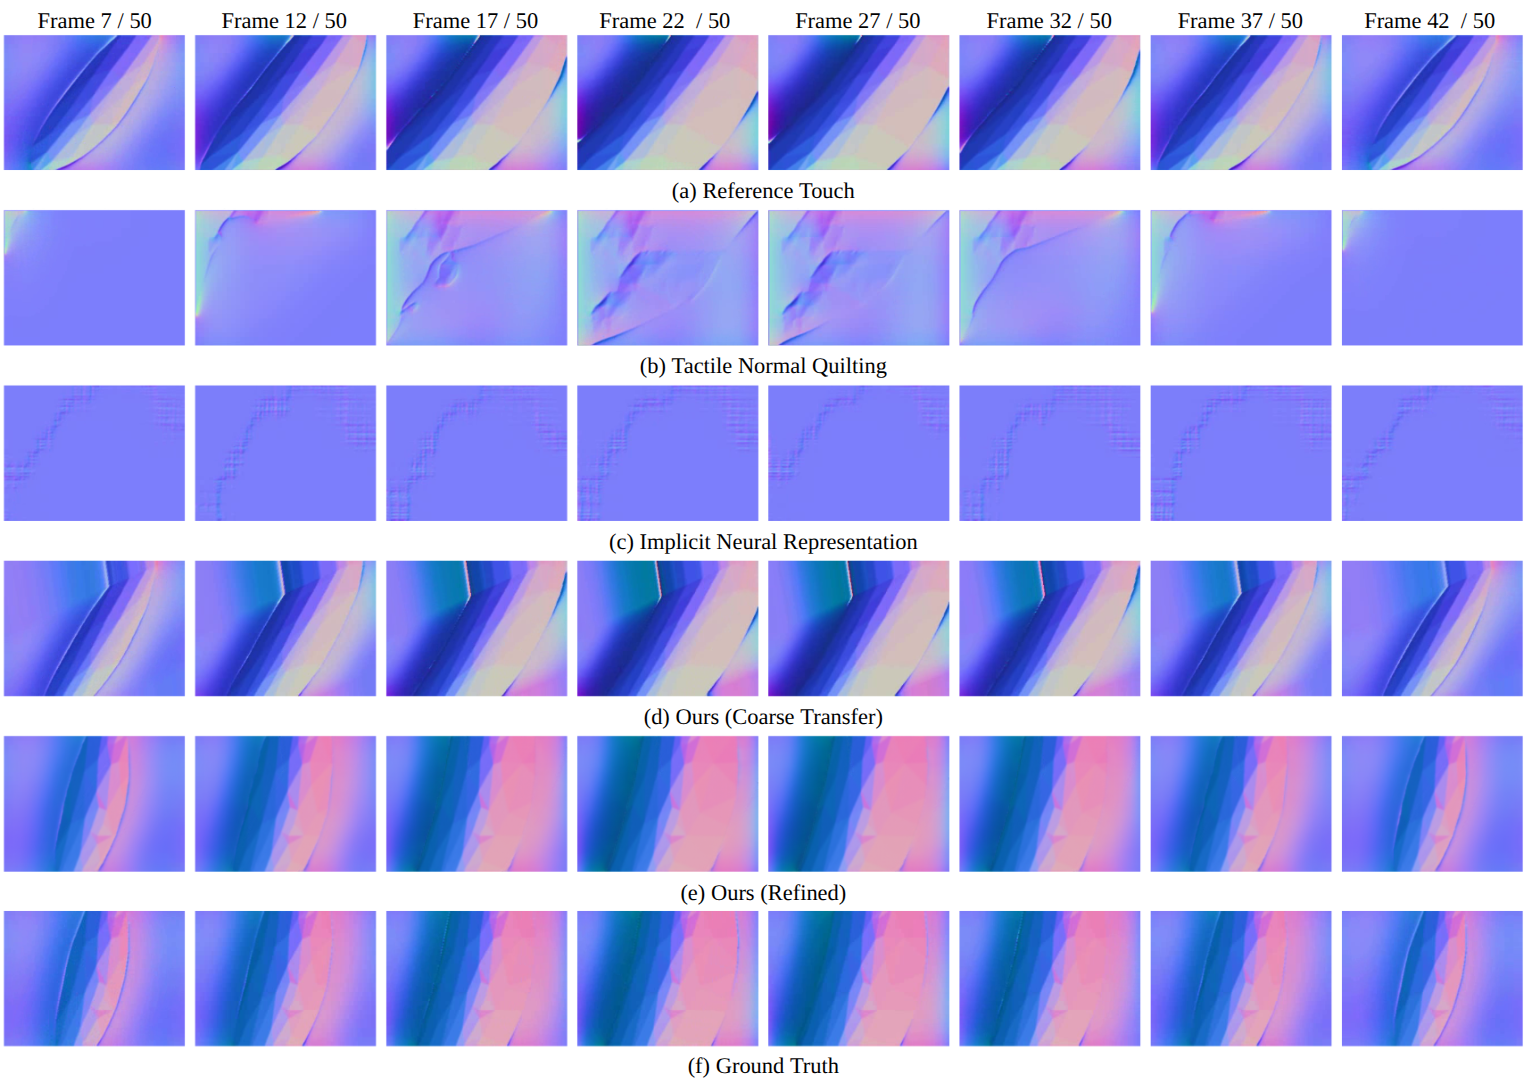
\includegraphics[width=\linewidth]{figures/full_pipeline_comparison.pdf}
  \rule{\linewidth}{7.0cm}% PLACEHOLDER -- remove when the real figure is dropped in
  \caption{\textbf{Comparison against baselines on the full pipeline benchmark.} Each row is one
    method and each column is a frame of the predicted tactile normal video, sampled across the
    press. The top row shows the reference tactile normal video that the prediction is transferred
    from. Baselines that predict a single tactile image rather than a video are shown with their
    prediction in the first column and marked \emph{N/A (image only)} thereafter, since they
    cannot express how the gel deforms over the press.}
  \label{fig:full_pipeline}
\end{figure*}
